\chapter{The Git structure}
\emph{Git}, as said before, is a distributed VCS.
It means that each user has a mirror of the repository (local
repository) and in the case of
\emph{git}, there is no need for a central server: each user is able to
fetch or push updates from other any other user repository (remote repository).
\emph{Git} is divided mainly in three components: the working directory,
the index, and the repository. The connection between these components
can be seen in Figure \ref{fig:git_structure}. Local and remote
repository have the same internal structure. What is a local
repository for an user is a remote repository for another user.

\begin{figure}[thp]
   \centering
   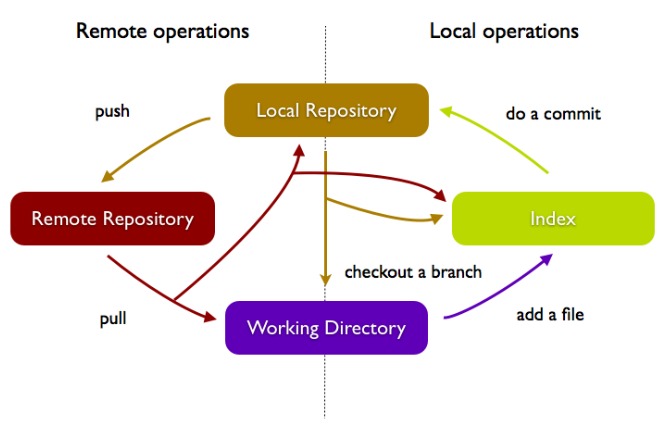
\includegraphics[width=0.8\textwidth]{images/git_workflow.png}
   \caption{Git Workflow}\label{fig:git_structure}
\end{figure}

\pagebreak

\section{The Repository}
\emph{Git} repository mirrors the evolution of a project during its lifetime. It is
the place where the snapshots taken during the project construction
are kept, as all the necessary information to
allow the users to navigate through all the snapshots. The snapshot's
structure and snapshots' relations are kept using, what is called, \emph{git
objects}. The information needed to go through the project is kept in,
what is called, \emph{git references}. In the next sections we
present both of them.


\subsection{Git Objects}
As we have presented before, \emph{git} keeps snapshots of how your system
looked like on a certain moment in time. This moment in time is
represented in \emph{git} by a commit. Each commit points to a tree
(corresponding to a directory), that
represents the structure of your project at that moment. So a tree
contains others trees and/or blobs. In \emph{git} the files are not stored as such. 
What \emph{git} keeps is an object called blob that represents the content of files. The
relation between the path of a file and the content of that path 
is kept on the trees corresponding to that path. \\

Figure \ref{fig:snapshot} presents an example of two snapshots. We
have two branches (the gray round square) pointing to two different
commits (the blue circles). The ''master'' branch is pointing to the
current commit, because it is identified by HEAD. It has as parent the commit ''ff12''
that is also pointed by the branch ''Foo''. We can see from the current
commit that when it was performed only the files ''file1.txt'' and the
''file3.txt'' were
in the index. It is also possible to see that in the root folder there was
a file called ''file3.txt'' and a folder called ''conn''. Inside this
folder there was a file ''file1.txt''.\\

In the next sections a detailed description about each object is
given, but for now something that is useful to know is that each
object is identified by a 40-character string. This string is
calculated by taking the SHA I hash of the contents of the object.
This approach has many advantages, being the two more important, in our
opinion, the
fact that it is possible to compare two objects only by comparing the hash and
if two objects have the same content then only one of them is kept.

\begin{figure}[h]
   \centering
   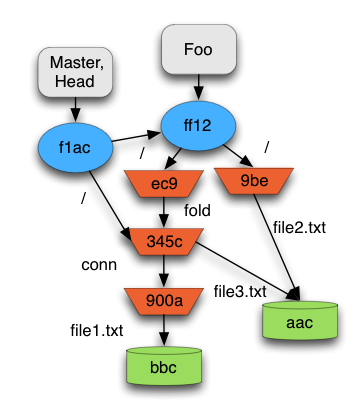
\includegraphics[width=0.4\textwidth]{images/object_assoc.png}
   \caption{A Snapshot}
   \label{fig:snapshot}
\end{figure}

\subsubsection{Blob}
A blob object, as said before, represents the content of a
file and the blob identifier is calculated from the blob content. So if we
have two files exactly with the same content, only one blob will be
stored, even if, they have different names. This happens because the
blob is not directly associated to a file. The relation between a path
(of a file) and a blob is kept in the tree object.  Figure \ref{fig:snapshot} 
shows an example of a blob representing two files.

\subsubsection{Tree}
A tree is nothing else than a map from names to blobs and other trees. Also here, a tree is not associated to any 
specific directory. If two directories have exactly the same content they will be
represented by the same tree object. Having the same content means
having exactly the same relations, or in other words, we
have exactly the same names in both trees and each name corresponds exactly
to the same objects in both trees. 

\subsubsection{Commit}
The commit object, is like a snapshot of the project on a certain moment in
time. A commit object has more variety of information than the two
objects addressed before. Looking a commit, it is possible to find out
the following:
\begin{itemize}
   \item Author - The person responsible for the change on the
   project.
   \item Committer - The person which actually created the commit. It
   is possible that the committer is different from the author. An
   author can create a patch, send it to the committer,
   which will create the commit.
   \item Parent - The previous commit, or, the commit from which this
   one was created. It is possible for this field to be empty, when 
   the commit is a Root Commit (the first commit to be done). 
   It is also possible to have two parents, when the commit is a result
   from a merge operation.
   \item Comment - It is mandatory, when creating a commit, to write a
   comment about the commit. Such comments should contain details about
   the changes that were done in the project.
   \item Tree - It is a pointer for a tree, or in other words, it is a pointer
   for how the project looked like on a certain moment in time. 
\end{itemize}

In our model, we concentrated our efforts in the Parent and in the
Tree fields. We just care about the structure of the object model, so,
we removed everything else that does not influences such
structure. One property that we observed when modeling, is that, we
cannot have cycles in the parent relation.

\subsubsection{Tag}
At last we have the tag object. The tag object is just a pointer to
a commit with some more information. It can be used to mark a special 
commit, like a new version of the project. The structure is quite 
similar to the commit object. It has a tagger (the person who created 
the tag), a date in which the tag was created, a message (some
comment from the tagger) and it points to a commit object. In our
model we did not model this object, because when abstracting it looks
like a branch, that we will see in next chapter.

\subsection{Git References}
Basically a reference is just a pointer to a commit. There is much
more about references, but in this manual we will focus on
Branches and the special reference HEAD.

\subsubsection{Branches}
One of the trump cards of \emph{Git} is its definition of branches. In other
VCS each time a branch is created a new copy of the entire repository
has to be done. Thus, branch operations in those VCS are slow and hard to use. 
In \emph{git}, when a new branch is created the only thing that
\emph{git} does is to create a new pointer to the current
commit. The current commit is marked by a special reference called
HEAD, that we present next.

\subsubsection{HEAD}
HEAD is maybe the most important reference in the repository. It
indicates where you are situated in the repository. When a commit is
done, \emph{git} has to know which commit is going to be the parent. 
It does so, looking into the HEAD. HEAD normally is a
pointer to a branch, so when the commit is done, the HEAD is kept, but
the branch points to the new commit. HEAD can identify directly a
commit, like for example, when a checkout is performed using a commit hash. But in this document lets keep it simple, HEAD will identify always a branch.

\section{Working Directory}

The working directory is basically a subset of
a file system that contains the files of the project you are
currently working on. These files can be the current files, files
retrieved from an old snapshot or even files that are not being
tracked. When retrieving an older snapshot of the project, the
working directory is updated to reflect the project in that state. The
untracked files in the working directory are just ignored, unless
there is a conflict when retrieving files from an older snapshot.\\

When a user starts a repository, all the files are untracked. When a
new file is created it will be untracked. So, how does \emph{git} know which
files are tracked or not? That is the role of index which we present
next.

\section{Index}
The index is something in between the working directory and the
repository. It has mainly two functions: to control which files are
being tracked, and to stage a file with the respective content to be
committed.\\

When a file is created, if the user wants that file to be
tracked it has to be added to the index. Each time the user modifies
the file's content and does not add it to index, the content in
index will diverge from the content in the working directory. The
file staged in index (file and respective content) is what is stored 
when a commit is created, irrespective of its current content in the
working directory.\\

It is important to notice that the index contains
just files. Directories are not tracked or staged, even if, the user
can still use the add operation with a
folder as parameter: instead of adding the folder to index, \emph{git}
recursively adds all the files
inside that folder to index.

